\subsection{Separation af tegn}
Separation af tegnene i nummerpladerne forgår i to trin: Først roterer vi billedet så nummerpladen ligger vandret. På denne måde blir det lettere at separere tegnene, da de kommer til at stå på en vandret linie med flugtende over- og underkanter. Selvom vi i vores afgrænsning af billedmaterialet har valgt at bruge billeder hvor nummerpladerne tilnærmelsesvis ligger vandret, har det vist sig, at de i praksis ofte er roteret så meget ,mellem $1^{\circ}$ og $3^{\circ}$, at vi får væsentligt mere ensartede nummerplader at arbejde med hvis vi korrigerer for dette. Som trin nummer to lokaliserer og isolerer vi tegnene i nummerpladen.

Rotationsmetoden returnerer hele det roterede originalbillede, mens separationsmetoderne returnerer syv enkeltstående billeder. Hvert billede er et tegn fra nummerpladen, skåret ud og omdannet til et binært billede.

\begin{figure}[htp]
\centering
\includegraphics[width=12cm]{system/illu/dia_trin2.png} 
\caption{Inddata, i form af ... , kommer ind i systemet i systemet fra højre. ..... Uddata er ....}
\label{fig:dia_trin2}
\end{figure}


\subsubsection{Rotation}
I dette afsnit beskrives det hvordan et billede af en nummerplade kan roteres, så nummerpladen optræder vandret i billedet. Metoden er blandt andet brugt i \cite{shapiro}.


\subsubsection*{Radon transformation}
%HELE DETTE AFSNIT ER MEGET TEKNISK. BURDE NOK VÆRE I IMPLEMENTATION. HER SKAL VEL IKKE STÅ SÅ MEGET MERE AND AT VI FINDER UD AF HVOR MEGET PLADEN ER VINKLET OG KORIGERER FOR DET.

En \textit{Radon transformation} beregner projektionen af et billede i flere forskellige retninger\cite{matlab_radon}. Denne type transformation kan bruges til at finde linier i billedet, og til at undersøge i hvilken retning disse linier går. Disse oplysninger er brugbare mht. rotation af et billede af en nummerplade, så denne plade står vandret i billedet.

%En Radon transformation er defineret således\cite{wiki_radon}: SKAL MÅSKE IKKE MED?

%UD MED DENNE:

%\begin{displaymath}
%		R[f](\alpha,s) = \int_{-\infty}^{\infty}f(x(t),y(t))dt \text{, hvor}
%\end{displaymath}
%\begin{displaymath}
%		(x(t),y(t)) = t(\sin\alpha, -\cos\alpha)+s(\cos\alpha,\sin\alpha)
%\end{displaymath}


%Radon transformation er en integral transformation, som kan transformere et to-domensionelt billede indeholdende linier til et andet domæne hvor liniernes placering og retninger kan beregnes\cite{toft_radon}. Vi vil dog ikke undersøge dette nærmere, blot bruge funktionen. ELLER NOGET?! Figur \vref{fig:radon_transform} viser hvordan Radon transformationen findes i en enkelt vinkel.

Vi vil undlade at gennemgå definitionen af Radon transformation. Idéen i en Radon transformation er dog illustreret i figur \vref{fig:radon_transform}. I denne ses det hvordan Radon transformationen laver en projektion af et billede i enkelt vinkel, $\theta$. 

%Kilden i en Radon transformation kan være enkeltstående eller en samling af flere. Den sidstnævnte model er den der bruges i dette tilfælde. Projektionen der foretages på et givent billede er et linært integrale hvor pixelenes intensiteter summeres i hver retning. %Figur \vref{fig:radon_transform} viser hvordan Radon transformationen findes i en enkelt vinkel ved brug af flere kilder.

\begin{figure}[htp]
  \centering
  \includegraphics[width=8cm]{system/illu/radon.png}
  \caption{En illustration af hvordan Radon transformation leder efter linier i en enkelt vinkel, $\theta$ udfra flere kilder (sources). Den blå firkant er billedet der undersøges. Pilene er sensorlinier (kilderne).\cite{matlab_radon}}
  \label{fig:radon_transform}
\end{figure}

Før en Radon transformation bruges til at finde linier og deres vinkler i et billede af en nummerplade, må kanterne i billedet detekteres. Dette giver en større chance for at Radon transformationen opfanger linierne i billedet. Når nummerpladens hældning i billedet er fundet, kan billedet roteres.

For at repræsentere et helt billede med en Radon transformation, udføres projektioner for alle vinkler mellem $0^{\circ}$ og $179^{\circ}$ (men ikke for $180^{\circ}$ da dette vil give samme resultat som ved $0^{\circ}$). Dette resulterer i en matrix der angiver i hvor høj grad det er sandsynligt at der findes en linie i original billedet for hver vinkel, $\theta$ samt sensorlinie. %I Figur \vref{fig:radon_matrix} er vist resultatet af en Radon transformation af et billede af en nummerplade.

%\begin{figure}[htp]
%  \centering
%  \framebox{\includegraphics[width=12cm]{system/illu/radon_matrix.jpg}}
%  \caption{Resultatet af en Radon transformation på et billede af en nummerplade. Jo lysere et område i denne matrix er, jo bla bla MANGLER DER EN SKALA???}
%  \label{fig:radon_matrix}
%\end{figure}

I Figur \vref{fig:Rotation} er vist et eksempel på et billede af en nummerplade, der roteres ved hjælp af Radon transformation. Bemærk at kun de horisontale kanter detekteres i det binære billede der viser kanter (mere om dette i afsnit \vref{sec:implementation/sep/rotation}).

\begin{figure}[htp]
  \centering
  \begin{minipage}[c]{6 cm}
    \framebox{\includegraphics{system/illu/rotate_example_input.jpg}}
  \end{minipage}\\
  \begin{minipage}[c]{6 cm}
    \framebox{\includegraphics{system/illu/rotate_example_edge.jpg}}
  \end{minipage}\\
  \begin{minipage}[c]{6 cm}
    \framebox{\includegraphics{illu/plate.jpg}}
  \end{minipage}
  \caption{Et billede af en nummerplade som roteres så den står vandret. Øverste billede forestiller originalbilledet, det midterste billede forestiller kant-detektionen mens det nederste billede er den roterede plade.}
  \label{fig:Rotation}
\end{figure}


\subsubsection*{Andre metoder brugt i litteraturen}
I det materiale vi har læst har vi ikke fundet beskrivelser af andre metoder til rotation end Radon transformation som er anvendt i \cite{sharpiro}. Vi er klar over at den lignende \textit{Hough transformation} eksisterer og at den også kan bruges til rotation, men vi har ikke arbejdet med den, da det virkede oplagt at bruge den åbenbart etablerede fremgangsmåde fra litteraturen. 

\subsubsection{Separation af tegn}

HEDDER DET SAMME SOM AFSNITTET OVENFOR

%Se nrpl.dk: Hvert af de op til 7 tegn på nummerpladen har et imaginært "felt" de kan brede sig i. Ikke alle tegn er lige brede, og generelt er bogstaver bredere end tal. "Feltet" til bogstaver er derfor bredere end feltet til tegn. Enkelte tegn er for smalle til at udfylde deres "felt", så designeren har fundet det hensigtsmæssigt at placere disse tegn visuelt centreret inden for deres "felt".

%"Således vil en nummerplade som MB 20 001 på grund af venstrestillingen af det sidste 1-tal have større mellemrum mellem højre kant og sidste tal end mellem venstre kant og første bogstav"


I det følgende beskrives to metoder til separation af tegn i en nummerplade. Disse to metoder arbejder med henholdsvis sammenhængende komponenter og såkaldt "signatur". I forbindelse med uarbejdelsen af metoden der bruger signatur viste det sig, at denne metode giver dårlige resultater. Derfor er kun metoden med sammenhængende komponenter blevet brugt i vores færdige system.

%HER BESKRIVER VI JO VORES SYSTEM, SÅ DET SKAL VÆRE KLART AT VI KUN BENYTTER EN METODE.

\subsubsection*{Metode: Sammenhængende komponenter}

MANGLER MÅSKE REFERENCER MELLEM BILLEDERNE.
Denne metode til at separere tegn i en nummerplade fungerer ved brug af sammenhængende komponenter. Ideén bygger på at hvert enkelt af de syv tegn som findes i billedet af nummerpladen er én sammenhængende komponent. De sammenhængende komponenter der arbejdes med her består altså af mørke pixels i originalbilledet (tegnene er sorte). Metoden bruges i \cite{nijhuis} og i \cite{kwas}.

For at tegnene skal udskille sig klart fra nummerpladens lyse baggrund er det nødvendigt at forstærke kontrasten i billedet. Ved en optimal kontrastforstærkning vil pixels som er en del af et tegn i et gråtonebillede af nummerpladen have intensitetsværdier som er meget mørke, mens eksempelvis pixels i den hvide nummerpladebaggrund vil have intensitetsværdier som er meget lyse. Et eksempel på kontrastforstærkning ses i figur \vref{fig:kontrast}.

% kontrast eksempel
\begin{figure}[htp]
  \centering
  \begin{minipage}[c]{8 cm}
    \framebox{\includegraphics{system/illu/eksempel_plade_gray.png}}\\
    \framebox{\includegraphics{system/illu/eksempel_plade_kontrast.png}}
  \end{minipage}
  \caption{Kontrast.}
  \label{fig:kontrast}
\end{figure}

Efter kontrastforstærkning oprettes et binært billede med sammenhængende komponenter. Sandsynligvis vil tegnene ikke være de eneste sammenhængende komponenter i billedet. Eksempelvis kan nummerpladen være beskidt eller der kan være mørke elementer uden for nummerpladen der vil være sammenhængende. Desuden kan det forekomme at tegn i nummerpladen "gror" sammen med pladens kant hvis der er snavs eller skruer mellem tegnet og kanten. Et eksempel på en nummerplade hvor nogle tegn er groet sammen med kanten ses i figur \vref{fig:skygge}.

MANGLER EKSEMPEL PÅ KOMPONENTER UDENFOR BILLEDET.

\begin{figure}[htp]
  \centering
  \begin{minipage}[c]{8 cm}
  	  \framebox{\includegraphics[width=7.75cm]{system/illu/skygge.png}}
	\end{minipage}\\
  \begin{minipage}[c]{8 cm}
  	  \framebox{\includegraphics[width=3.7cm, height=3.5cm]{system/illu/skygge-y.png}}
  	  \framebox{\includegraphics[width=3.7cm, height=3.5cm]{system/illu/skygge-6.png}}
	\end{minipage}
	\caption{Et eksempel på et billede af en nummerplade, som er repræsenteret ved sammenhængende komponenter (de hvide områder repræsenterer komponenter), hvor tegnene \textbf{Y} og \textbf{6} er groet sammen med pladens kant. Det øverste billede er hele nummerpladen mens de to nederste er forstørrelser af henholdsvis området omkring \textbf{Y}'et og \textbf{6}-tallet. Bemærk de tynde hvide streger der forbinder de to tegn med kanten af pladen.}
  \label{fig:skygge}
\end{figure}

%EKSEMPEL MED SKYGGER: DER ER TO SLAGS!

%SVAG BELYSNING OVENFOR ER IKKE RIGTI TIL AT FORSTÅ. FOR LØST? VI KAN VEL BARE SIGE AT DER ER ANDRE MØRKE OMRÅDER UDEN FOR PLADEN.

%DET ER LETTERE AT FORSTÅ HVIS MAN TALER OM SORT OG HVID I STEDET FOR SPECIFIKKE INTENSITETSVÆRDIER. DER STÅR JO IKKE NOGEN FORKLARING TIL DEM.
%Figur ?? viser forskellen på et billede af en nummerplade uden kontrast og et med hvor kontrasten i billedet er forstærket.

 %I figur \vref{fig:concomp} ses et billede af en nummerplade hvor de sammenhængende komponenter er hvide. Eksemplet viser en situation som beskrevet ovenfor, hvor det ikke kun er tegnene der er sammenhængende komponenter.

%DETTE SKAL MÅSKE UD, DA VI JO TIDLIGERE HAR VIST ET LIGNENDE EKSEMPEL?

%\begin{figure}[htp]
%  \centering
%  \framebox{\includegraphics[width=8cm]{system/illu/concomp_example.png}}
%  \caption{Illustration af sammenhængende områder i en nummerplade. De sammenhængende områder er vist som hvide i dette binære billede.}
%  \label{fig:concomp}
%\end{figure}

Ud fra følgende regler, vælges de sammenhængende komponenter der kan være tegn:

\paragraph{1. Hvert tegn fylder maksimalt $\frac{1}{7}$ af billedets areal:} Da en nummerplade består af syv tegn og noget baggrund vil ingen tegn fylde mere end $\frac{1}{7}$ af billedets areal. 
\paragraph{2. Hvert tegn har en maksimal bredde på $\frac{1}{7}$ af billedets bredde:} Denne regel er lavet ud fra samme argument som ovenfor.
%\item Tegnenes højde er større end deres bredde. DETTE GØRES IKKE!
\paragraph{3. Tegnenes minimale højde skal være mindst en vis konstant:} Da der vil være støj i form af meget små komponenter, sættes der en grænse for hvor lavt et tegn kan være.% (her: 5 pixels)
\paragraph{4. Tegnenes minimale størrelse skal være mindst en vis konstant:} Samme som ovenfor: en grænse for hvor lille et tegn kan være.% (her: 5 pixels)
\paragraph{5. For hvert tegn findes der seks andre tegn som er omtrent ligeså høje som det pågældende tegn:} Alle tegnene i pladen er lige høje.
\paragraph{6. For hvert tegn findes der seks andre tegn som befinder sig i omtrent samme højde som det pågældende tegn:} Hvis nummerpladen står vandret i billedet, vil alle tegn være i samme højde.
\paragraph{7. De syv tegn er opdelt i tre grupper:} I forhold til afstanden mellem tegnene danner de to bogstaver, de to første tal samt de tre sidste tal hver især en gruppe.

%VI BØR NOK LAVE LISTEN OM TIL NUMMEREREDE PARAGRAFER MED MERE UDFØRLIGE BESKRIVELSER.


Når de sammenhængende komponenter der ikke kan være er sorteret fra fås et binært billede hvor kun tegnene i nummerpladen er markeret. Figur \vref{fig:sorterede-concomp} viser et eksempel.

\begin{figure}[htp]
  \centering
  \framebox{\includegraphics[width=8cm]{system/illu/concomp_kun_bogstaver.png}}
  \caption{Et eksempel på et binært billede af en nummerplade, hvor kun tegnene er markeret.}
  \label{fig:sorterede-concomp}
\end{figure}

Til sidst udklippes de komponenter der resterer (tegnene). Et eksempel på syv udklippede tegn er vist i figur \vref{fig:tegn-udklip}.

\begin{figure}[htp]
  \centering
  \begin{minipage}[c]{8 cm}
  	  \framebox{\includegraphics[height=1cm]{system/illu/char1.png}}
  	  \framebox{\includegraphics[height=1cm]{system/illu/char2.png}}
	  \framebox{\includegraphics[height=1cm]{system/illu/char3.png}}
  	  \framebox{\includegraphics[height=1cm]{system/illu/char4.png}}
	  \framebox{\includegraphics[height=1cm]{system/illu/char5.png}}
  	  \framebox{\includegraphics[height=1cm]{system/illu/char6.png}}
	  \framebox{\includegraphics[height=1cm]{system/illu/char7.png}}
	\end{minipage}
  \caption{Et eksempel på syv billeder af syv tegn, som er klippet ud fra en nummerplade.}
  \label{fig:tegn-udklip}
\end{figure}

\subsubsection*{Metode: Bjerg/dal}
Denne metode baseres på en projektion af kolonnerne i en nummerpladen. Det vil sige at intensitetsværdierne i hver kolonne summeres og udfra disse summer laves en "signatur". Denne projektion vil, med en lys nummerplade med mørke tegn, give os en indikation af hvor der er tegn (bjerge) og de lyse områder mellem tegnene (dale), hvorefter vi kan udskærer tegnene. Metoden kaldes "peak-to-valley" på engelsk og bruges i \cite{ron} og \cite{kwas}.

%Som i metoden med sammenhængende komponenter er det en fordel at forstærke kontrasten i billedet. HVORFOR?

Nummerpladens signatur fås ved at summere projektionerne af alle rækkerne i billedet. Hvis denne signatur præsenteres som en graf i et koordinatsystem vil der forekomme toppe i de kolonner hvor der høj intensitet. Idéen er så at udvælge de otte højeste toppe som de otte steder i x-planen der skal skæres ved. Dette er illustreret i figur \vref{fig:ptv-signatur}.

\begin{figure}[htp]
  \centering
  \framebox{\includegraphics[width=10cm]{system/illu/signatur.png}}
  \caption{FIGUR AF SIGNATUR-KONCEPT}
  \label{fig:ptv-signatur}
\end{figure}

\subsubsection{Metoder fra litteraturen}

Vi har ikke fundet andre metoder til separation af tegn end de to nævnte. Det kan dog nævnes at man i \cite{parker} og \cite{kwas} bruger sammenhængende komponenter i arbejdet med at lokalisere nummerpladen. I denne proces ses det på om der er et vist antal sammenhængende komponenter inde i den nummerpladekandidat man har fundet.

%NOGEN FINDER LOKALISERER NUMMERPLADERNE VED HJÆLP AF ANALYSE AF CONNECTED COMPONENTS. DET MINDER JO OMDET DU GØR, MEN DE GØR DET BARE TIDLIGERE. IKKE ANDRE?

%%%%%%%%%%%%%%%%%%%%%%%%%%%
% Note fra segmentering af tegn
%%%%%%%%%%%%%%%%%%%%%%%%%%%%


\begin{comment}
\subsubsection*{Skan-linie}

Bruges ikke da det er for mange felter som bliver valgt. Kan måske gøres bedre ved filtrering før???

Først gøres billedet sort-hvis med im2bw. Her kan grænseværdi bestemmes med greythresh. Virker måske bedre at sætte grænseværdien lavt, så meget af billedet bliver hvidt.

Billedet skal skæres foroven og forneden. Dette gøres simpelt ved at finde den største pixl-sum i toppen af billedet og den største sum i bunden. Det antages så at disse max-summer er dele af nummerpladerne hvor teksten ikke er startet.

Step igennem vertikale linier: hvad sker før tegn, i et tegn, i slutningen af et tegn og efter et tegn.
\end{comment}


%%%%%%%%%%%%%%%%%%%%%%%%%%%
% Beskrivelser af PDfer
%%%%%%%%%%%%%%%%%%%%%%%%%%%%


\begin{comment}
\subsubsection*{Noter fra møde med Søren 20/2:}
identifikation: Se på en pixel, har naboer en kontrast farve?
En scan-linie: hvordan varierer kontrasten henover linien?
Adaboost - godt










\subsubsection*{cano.pdf}
Bruger kun gråtone info. Arbejder også med nummerplader som skal være læsbar for det menneskelige øje.

Metode:
Histogram - først normaliseres billedet
Sobel filter - fremhæver ikke-homogene områder
"A simple threshold and a sub-sampling" bruges til at vælge områder der kan være nummerpladen

Husker alle områder som kan være nummerplader så de forkerte først vælges fra i genkendelses-fasen. Bruger multi-hypothesis detection (ikke forklaret yderligere i teksten).

Feature vektorer: hver pixel i et træningsbilleder er blevet klassificeret som positiv (del af nummerplade) eller negativ (ikke del af nummerplade). Minimerer efterfølgende det negative sæt.

Bruger kd-træ data struktur og en "omtrent nærmeste nabo" søgeteknik.

\subsubsection*{ron}

* Find de gule (hos os: hvide) områder i billedet
* Forstør disse områder
* Find vinklen på nummerpladen ved brug af "Radon transform"
* Justering af nummerpladens konturer
* Unødvendige dele af billedet fjernes (kun nummerpladen tilbage)
* Billedet i gråtone, herefter gøres det binært
* Billedet normaliseres
* Tegn-inddeling vha. peak-to-valley

De brugte Matlab. De havde følgende relevante problemer og løsningsforslag til disse:

* Udtrækning af det gule område giver ofte fejl. Man kunne supplere denne udtrækning med en algoritme der indberegner at nummerplader har en klar signatur idet der er stærke grå-tone variationer i regulære intervaller (henover nummerpladen, mener de vel?)

* Hvis der er flere nummerplade-kandidater i billedet skal hver af dem testes.

\subsubsection*{nijhuis.pdf}

Bruger regler for nummerplader i systemet

    * Starter med kontrast “udstrækning”, bortfiltrering af støj (der tages selvfølgelig højde for billedkvaliteten i denne del)
    * Lokalisering af nummerpladen: fuzzy clustering algoritme som bruger karakteristikker som “gul-hed” og teksturer
    * Gul-hed er defineret af frekvenstabel lavet fra manuelt udklippede nummerplader
    * Tekstur: her ser man på grå-værdien af de 8 nabopixels
    * “global threshold” baseret på gennemsnitsværdien af gråtone: fås binært billede
    * Udfra regler (højde, bredde m.m) findes potintielle tegn
    * Nummerpladen gives kun videre til mønstergenkendelse hvis den indeholder det rette antal tegn

Dette system godkender 75\% af billederne. Problemer med skruer i nummerpladen. Problemer med global threshold – burde gøres på pr-tegn-basis.

\subsubsection*{parker.pdf}

Der bruges en algoritme der først lokaliserer elementer der kan være tegn/bogstaver hvorefter den udvælger et område som nummerplade

* Konverter til gråtone billede
* 5x5 filter, fjerne støj
* Find kanter i billedet vha. Shen-Castan kant-detektor
* Gør billedet binært og del elementer i forgrunden fra hinanden
* Algoritme der finder bogstaver på baggrund af forskellen i gråtone værdien af bogstav/baggrund
* Områder hvor der ikke er (det rette antal) bogstaver udelukkes
* For at finde nummerplade bruges genetisk algoritme der bedømmer rektangler med tegn: har de den rette størrelse? er bogstaverne korrekt placeret i rektangel? osv.
* Algoritmen vægter hvert område og filtrerer til sidst i disse områder udfra deres vægt

Stort problem: svært at finde tegn.

\subsubsection{kwas.pdf}
Billedet skiftes til farverummet YUV fra vilket luminans er det eneste der bevares. Herefter normaliseres billedet (Hele den diskerete "range" udnyttes). Kigger på skift i kontrast. Gælder alle nummerplader. Finder alle tekster. Den rigtige skal vælges.

Identifikation af plader:

1. "Connected components analysis" (der kigger på et binært billede?) vælger områder med høj kontrast (threshold). De fundne områder undersøges og områder elimineres efter regler i pdf.  Herefter, er der lignenede grupper i nærheden af funden gruppe? Måske er der en serie tegn dvs. en sætning = plade.

2. Searching for signatures of license plates. Et karakteristisk skift i luminans i en linie i billedet.

Potentielle plader roteres så de er vandrette.

Segmentering af tegn:
Scan af peaks og valleys samt analyse af sammenhængende grupper fra identifikationsprocessen sammenlignes og segmentering foretages.

Mønstergenkendelse foregår med neuraltnetværk.

\subsubsection{shapiro.pdf}
For at sætte hastigheden op foretages visse operationer på kraftigt nedsamplede billeder. Finder lodrette linier. Bruger Robert's edge detector til at fremhæve dem (Tegner den på billedet?). Dette efterlader en masse lodrette linier i området med nummerpladen. Et Rank filter? bruges på billedet. Efterlader en lys elipse i det område hvor pladen findes. Scanner billedet lodret for at finde det lyseste område og klipper ud (Klipper et noget større område end pladen ud på eksemplet i pdf'en). Der er formler i beskrivelsen. Roter pladen hvis skæv (Formler i pdf). Nohet med at finde linier i billedet og rotere stlsvarende (Hough og Radon transform). Det er først når vi skal genkende tegnene på pladen vi bruger billedet i sin originale opløsning.
\end{comment}


